\subsection{Grobkonzept 4} \label{subsec:grobkonzept3}
\begin{table}[H]
\footnotesize
\begin{tabular}{>{\HY\RaggedRight}p{3cm} >{\HY\RaggedRight}p{2.2cm} >{\HY\RaggedRight}p{4cm} >{\HY\RaggedRight}p{3.3cm} >{\HY\RaggedRight}p{1.2cm}}
\hline
	\textbf{Bestandteil}		&\textbf{Typ}			&\textbf{Funktion}									&\textbf{Specs}			&\textbf{Anz.}\\
	\hline
\rowcolor{dgelb}
\multicolumn{5}{l}{\textbf{Stromerzeugung}}\\
	Wasserlift 				& 						&Umwandlung in Rotationsenergie						&							&5	\\
	Generator				&AC						&Umwandlung in elektrische Energie					&???							&5	\\
\rowcolor{dblau}
\multicolumn{5}{l}{\textbf{Elektrotechnik}}\\
 	Wechselrichter			&						&Einspeisung ins Stromnetz							&							&1	\\
\rowcolor{dpink}
\multicolumn{5}{l}{\textbf{Bedienung}}\\
 	Anzeige 					&Display					&zeigt Tankfüllstände und Generatordaten an 			&							&1	\\
\rowcolor{dgruen}
\multicolumn{5}{l}{\textbf{Abwassertechnik}}\\
Bypass						&Absperrklappe			&Umleitung für Wartungsarbeiten am Wasserlift 		&							&6\\
Bypass 						&in Wirklichkeit			&sind es viel mehr als 6								&5*13+16=					&81\\
Leitung						&						&für Wartungsarbeiten 								&							&1\\
\hline
\end{tabular}
\end{table}
Im Grobkonzepts 4 wird die potenzielle Energie des Abwassers mit der Wasserlifttechnik ausgenutzt. Das Abwasser fliesst in eine Schaufel und wird in der Schaufel im Rohr nach unten transportiert. Somit erhält der Lift eine Bewegung nach unten und entleert am tiefsten Punkt das Abwasser. Die Leitung ist nie komplett mit Wasser gefüllt, daher kommt es zu einem Luftwiderstand in der Leitung, der das Abwasser abbremst.
\newpage
\begin{wrapfigure}{r}{0.5\textwidth}
  \begin{center}
    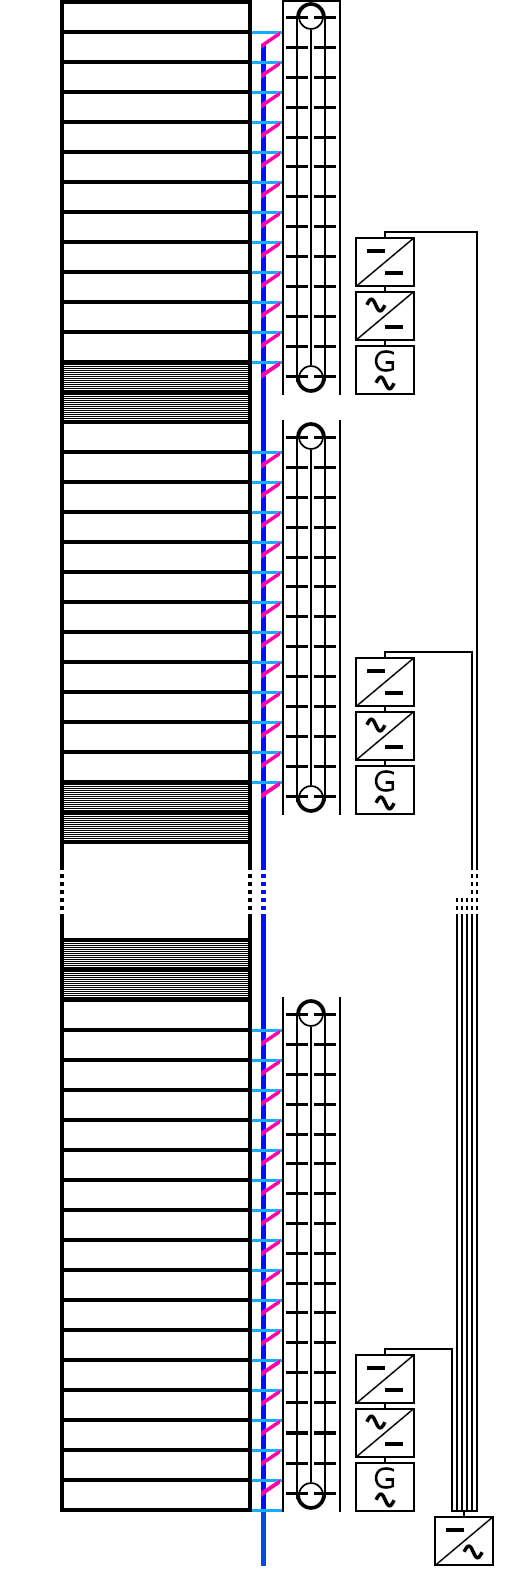
\includegraphics[width=0.48\textwidth]{grobkonzept4}
  \end{center}
  \caption{Grobkonzept 4}
\end{wrapfigure}
Die 5 oberen Lifte haben eine Länge von 66.08m, der unterste Lift 80.24m. Für Wartungsarbeiten existiert eine zusätzliche Leitung, die mittels Bypass angesteurt wird.

\textbf{Vorteile:}							\newline
+	kostengünstig							\newline
											\newline
\textbf{Nachteile:}\newline
-	defekt anfälliger						\newline
-	umbau									\newline
-	Verstopfungsresistent					\newline	
\WFclear			
\newpage